%%%%%%%%%%%%%%%%%%%%%%%%%%%%%%%%%%%%%%%%%%%%%%%%%%%%%%%%%%%%%%%%%%%%%%%%%%%%%%%%
%2345678901234567890123456789012345678901234567890123456789012345678901234567890
%        1         2         3         4         5         6         7         8

\documentclass[letterpaper, 10 pt, conference]{ieeeconf}  % Comment this line out if you need a4paper

%\documentclass[a4paper, 10pt, conference]{ieeeconf}      % Use this line for a4 paper

\IEEEoverridecommandlockouts                              % This command is only needed if 
                                                          % you want to use the \thanks command
\usepackage{subfigure}
\usepackage{cite}
\usepackage{amsmath,amssymb,amsfonts}
% \usepackage{algorithmic}
\usepackage{graphicx}
\usepackage{textcomp}
\usepackage{xcolor}
%\usepackage[numbers,sort&compress]{natbib}
\usepackage{algorithm} %format of the algorithm 
\usepackage{multirow} %multirow for format of table 
\usepackage{amsmath} 
\usepackage{gensymb}
\usepackage{mathtools}
\usepackage{forloop}
\usepackage{soul}
\usepackage{caption}

 
\usepackage{algorithmicx}  
\usepackage{algpseudocode}  

\usepackage{algorithm}  
\usepackage{graphics}
\usepackage{booktabs}  
\usepackage[UTF8]{ctex} 



\soulregister\cite7
\setlength{\textfloatsep}{5pt}

\overrideIEEEmargins                                      % Needed to meet printer requirements.

%In case you encounter the following error:
%Error 1010 The PDF file may be corrupt (unable to open PDF file) OR
%Error 1000 An error occurred while parsing a contents stream. Unable to analyze the PDF file.
%This is a known problem with pdfLaTeX conversion filter. The file cannot be opened with acrobat reader
%Please use one of the alternatives below to circumvent this error by uncommenting one or the other
%\pdfobjcompresslevel=0
%\pdfminorversion=4

% See the \addtolength command later in the file to balance the column lengths
% on the last page of the document

% The following packages can be found on http:\\www.ctan.org
%\usepackage{graphics} % for pdf, bitmapped graphics files
%\usepackage{epsfig} % for postscript graphics files
%\usepackage{mathptmx} % assumes new font selection scheme installed
%\usepackage{times} % assumes new font selection scheme installed
%\usepackage{amsmath} % assumes amsmath package installed
%\usepackage{amssymb}  % assumes amsmath package installed



\title{\LARGE \bf
带死亡判断的车辆换道研究——基于强化学习和注意力机制
}

\author{沈炼成,林镇阳,韩立君\thanks{沈炼成(2021E8014682015),林镇阳(202118020629020),韩立君(202118020629022)来自中国科学院大学,人工智能学院,北京。    } }% <-this % stops a space


%\UseRawInputEncoding
\begin{document}



\maketitle
\thispagestyle{empty}
\pagestyle{empty}


%%%%%%%%%%%%%%%%%%%%%%%%%%%%%%%%%%%%%%%%%%%%%%%%%%%%%%%%%%%%%%%%%%%%%%%%%%%%%%%%
\begin{abstract}
本文主要针对车辆换道问题进行研究,提出含死亡判断的D3QN算法,结合ego-attention和non-local block。选择图像与向量的混合形式作为输入,成功实现了超车换道。同时本文针对不同输入、不同训练奖励,不同算法以及是否加入死亡判断进行了大量的对比实验,实验结果证明我们的方法表现最优同时具有较高的稳定性。

\end{abstract}

\begin{keywords}
    强化学习,超车换道,D3QN
\end{keywords}


%%%%%%%%%%%%%%%%%%%%%%%%%%%%%%%%%%%%%%%%%%%%%%%%%%%%%%%%%%%%%%%%%%%%%%%%%%%%%%%%
\section{简介}

自动驾驶已经被广泛认为是改变交通系统的最重要的方式之一,例如其可以减少因人为不当操作带来的交通事故或者缓解交通阻塞\cite{FAGNANT2015167}。
然而自动驾驶车辆在复杂环境中正确驾驶仍然具有挑战性。

通常一个自动驾驶系统包含四个模块:环境感知模块,决策模块,控制模块,驱动模块\cite{li2018reinforcement}。决策模块的任务是根据来自感知模块的传感器信息做出合适的驾驶决策,然后规划出一条可行驶的路径给控制模块。如何做出合适的换道决策已经
当前的热门研究领域之一,一些研究关注车辆的有效变道轨迹规划\cite{xu2012dynamic,yang2018dynamic},另外一些研究则强调跟踪规划轨迹所需要的控制器\cite{cesari2017scenario,suh2018stochastic}。最近的研究则是通过实际的自然驾驶数据以学习或者模仿人类驾驶员的车道变换\cite{wang2014investigation,li2017retrieving,xu2018naturalistic},也有研究者利用端到端的技术直接建立感知数据到
换道决策行为的映射关系\cite{jeong2017end}。

除上述方法外,强化学习也已广泛应用于自动驾驶决策任务,例如车道保持\cite{oh2000new,sallab2016end}和自主巡航\cite{desjardins2011cooperative},因为它具有处理时序问题和寻求长期目标的最优策略的能力。在换道任务中,强化学习模型主要接受邻近车辆的状态数据或者图像数据作为输入\cite{li2019reinforcement,wang2019lane},并产生车辆换道决策输出。
在本工作中我们着重研究车辆的状态的空间是如何表示的,当前两种使用最广泛的状态空间表示方法都有不同的缺点:一方面,基于向量的状态空间表示对不同道路结构的泛化性能不足并且不能找到对自动驾驶车辆的换道决策有更加显著影响的邻近车辆。另一方面,基于图像的状态空间表示不能很好表示车辆的速度等信息并且同样
没有考虑空间位置关系和车辆间的相互作用。

注意力机制的引入使得神经网络能够发现可变数量的输入中的相互依赖性,可以很好地解决上述问题。在Sadeghian 等\cite{sadeghian2018car}的研究中,使用了道路的鸟瞰图的注意力机制来进行汽车轨迹预测,\cite{vaswani2017attention}已经开发了用于句子翻译的多头注意力机制,\cite{messaoud2019non}提出了适合用于图像输入的非局部多头注意力机制,\cite{leurent2019social}
中则提出了能够捕获当前车辆和周围车依赖关系的自注意力模型,适合用于向量输入。
本文中主要分析了不同状态表示下结合注意力机制对自动驾驶换道任务的影响。

我们的工作主要如下:首先,我们利用合适的双输入状态表示,结合局部鸟瞰图图像与向量输入,并且在每个输入分支应用不同的注意力机制,使得在智能体决策过程中以更大的权重考虑关键交互车辆,从而提升了深度强化学习的性能;
此外,我们对不同状态表示、奖励函数形式、强化学习算法进行了一系列消融实验,实验表明此类网络结构对自动驾驶车辆在换道任务中的性能有较大提升,其能够以视觉上可解释的方式捕捉环境中车辆的交互模式。


\section{任务描述与分析}

\subsection{任务描述}

整体任务为根据输入的车辆周围情况,借助深度强化学习算法得到高层的指令规划。再借助仿真器内部的运动规划器,将高层指令转化为具体的轨迹让底层控制器有效跟踪。最终实现汽车的超车换道。评价标准如下:
\begin{itemize}
    \item 尽可能少碰撞
    \item 尽量保持车道线内平稳行驶
    \item 速度越快越好
    \item 有前车阻挡能尝试安全换道
\end{itemize}

\subsection{仿真环境描述}
整体实验基于$highway\_env$\cite{highway-env}开发,具有较强的灵活性。下面分别针对状态空间、动作空间等进行叙述。

\subsubsection{状态空间}
在环境中,状态空间可以选择底层的低维向量输入,也可以选择高维的图像输入和占用格作为输入。下面重点叙述使用低维向量输入和图片输入的基本情况。

当使用低维输入时,传入15辆车的坐标、速度、倾斜角度等信息表示出来,包括$x,y,vx,vy,cos_h,sin_h$。传入一个大小为$(15,7)$的数组。方便后面网络进行处理,其中第一行表示的是本车的的各种信息。

使用图片输入时,传入大小为$(600,150)$的图片,同时将图片转化为灰度图。由于一张图片难以获得车辆的完整信息(如速度、运动方向等难以推测),因此将过去4帧叠放在一起作为状态观测输入,便于从观测推出状态。

\begin{figure}[htb] %H为当前位置,!htb为忽略美学标准,htbp为浮动图形
    \centering %图片居中
    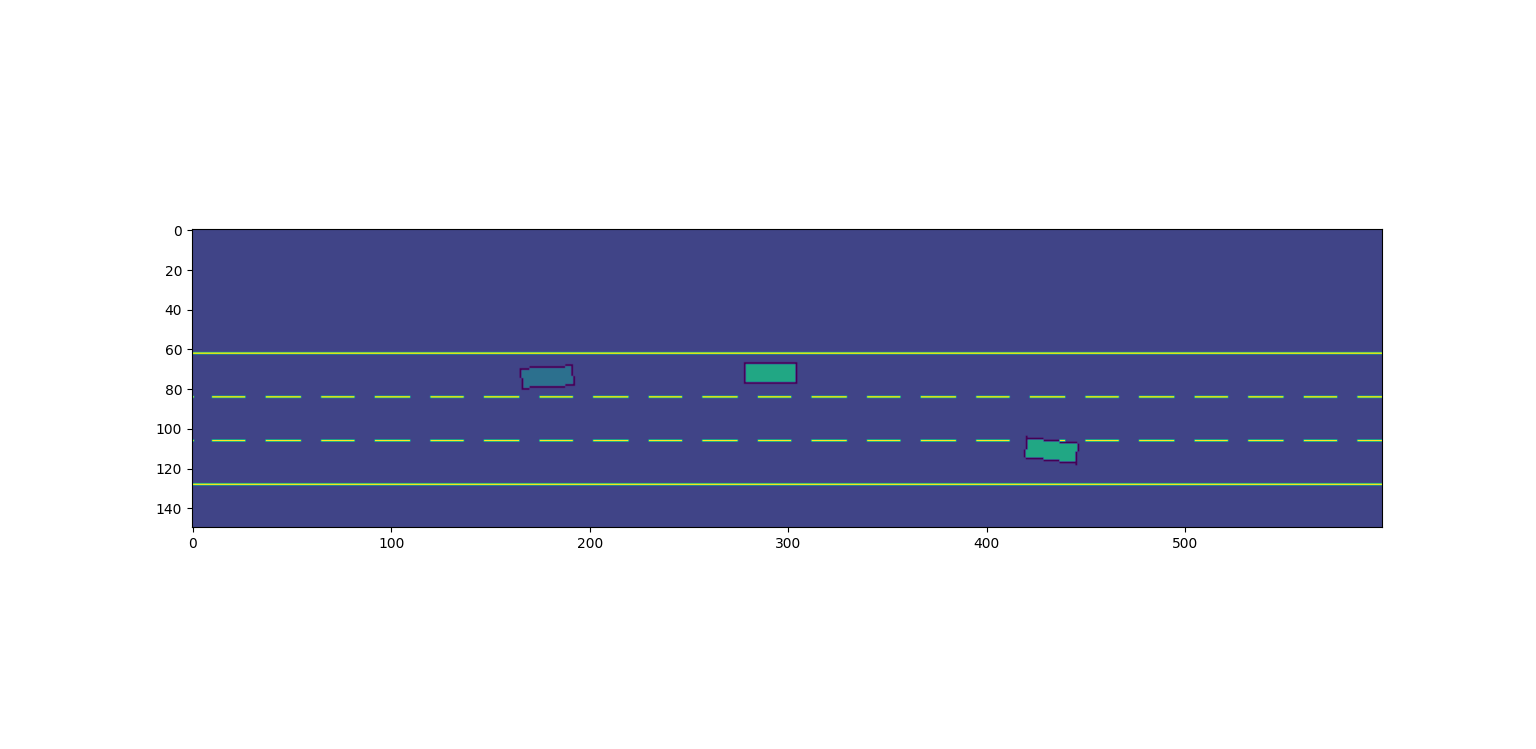
\includegraphics[width=0.5\textwidth]{fig/1.png} %插入图片,[]中设置图片大小,{}中是图片文件名
    \caption{图像输入} %最终文档中希望显示的图片标题
    \label{Fig.main1} %用于文内引用的标签
\end{figure}

后续实验证明,向量输入的归一化以及将两者信息整合同时输入可以显著提升换道效果。

\subsubsection{动作空间}
仿真环境可以将动作设置为连续的油门和方向盘角度,但连续空间训练收敛难度会增大。考虑到算力限制,因此使用离散动作进行控制,再将离散动作送入规划器中生成连续动作。在仿真器中,可以分为5个离散动作——左转、保持车道、右转、加速、减速。分别用动作$a_0$到$a_4$表征。这五个动作共同构成了仿真环境的动作空间,下层规划器根据决策指令对车辆动作进行规划控制。

\subsubsection{奖励设置}
环境中奖励设置较为灵活,主要分为三个部分,碰撞惩罚、车速奖励、靠右奖励。系统默认碰撞惩罚为-1,无碰撞为0。车速奖励为$r_v = 0.4\frac{(v_t-v_{min})}{(v_{max}-v_{min})}$其中,$v_{max} = 30m/s,v_{min}=20m/s$。此外还有靠右奖励,奖励系数为0.1。后面我们会讨论调整奖励系数对车辆的影响,实验发现,删除靠右奖励会导致车辆换道次数显著增加。

\subsection{任务分析}
根据任务需要我们设计强化学习算法,将低维或高维输入转化为离散的汽车换道决策指令。即首先需要对观测量进行提取推测,得到状态量。再将状态量作为输入得到动作。而近来深度强化学习的兴起让这两个环节可以直接联合训练,提升了学习效率。

在学习算法方面,我们采用了Dueling DDQN技术加入了一些训练技巧,能够有效提升收敛速度和训练稳定性。具体方法我们会在下节进行详细叙述,同时与之前的Dueling DQN,DQN进行比较,证明我们方法的有效性。同时针对输入,我们分别探讨了对于向量输入、图片输入和混合输入的效果。此外,针对不同奖励设置进行了消融实验。

\section{强化学习算法}
可以将超车换道问题转化为一个马尔可夫问题,由$<\mathcal{S},\mathcal{A},\mathcal{P},\mathcal{R},\gamma>$来表示,分别代表了状态空间、动作空间、转移概率、奖励函数、折扣因子。

根据前一节的分析,状态空间、动作空间、奖励函数均已得到。折扣因子$\gamma$设为0.99。不妨设$t$时刻的回报$G_t$为:
\begin{equation}
    G_t = \sum^{\infty}_{i=0}\gamma^ir_{t+i}
\end{equation}

$G_t$表示了从$t$时刻到结束的总的奖励,整个强化学习过程的目标即为最大化回报。但转移概率未知,因此采用无模型强化学习的方法,常用的无模型方法为Q学习算法。针对某个策略,定义$Q^\pi$为状态动作对好坏的评价标准,可以借助前面的回报定义为:

\begin{equation}
    Q^\pi = \mathbb{E}_\pi[G_t|s_t=s,a_t=a]
\end{equation}

同时使用经验回放池,使得训练数据满足独立同分布假设,以及充分利用过往探索经验,方便进行深度学习。使用目标网络,防止计算TD误差时目标变动导致更新困难。使用$\epsilon-greedy$算法,$\epsilon$值逐渐衰减,来平衡整个利用与探索的过程。整个DQN算法\cite{mnih2015human}流程如下所示:

\begin{figure}[htbp] %H为当前位置,!htb为忽略美学标准,htbp为浮动图形
    \centering %图片居中
    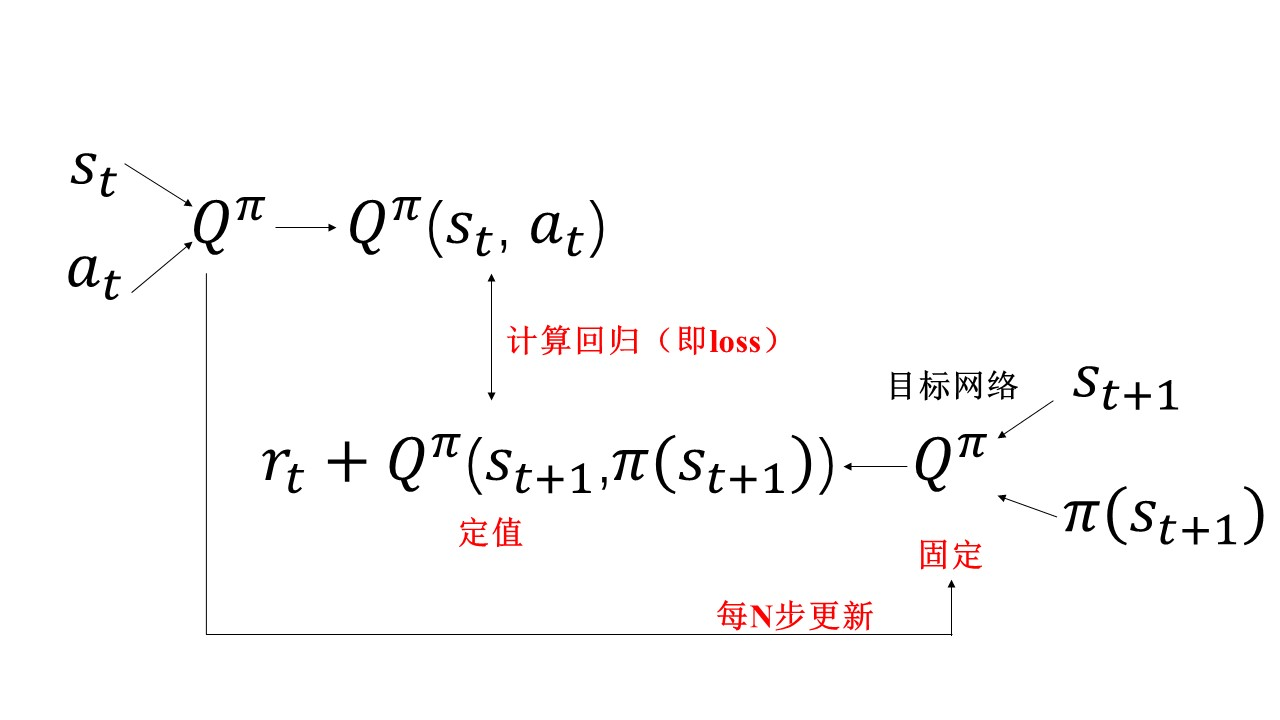
\includegraphics[width=0.5\textwidth]{fig/2.JPG} %插入图片,[]中设置图片大小,{}中是图片文件名
    \caption{DQN算法框架\cite{mnih2015human}} %最终文档中希望显示的图片标题
    \label{Fig.main2} %用于文内引用的标签
\end{figure}


但是传统的DQN算法会存在Q值过高估计的问题,因此引入了Double DQN\cite{van2016deep},将决策动作生成网络和状态动作对估值网络分开,可以一定程度缓解过估计问题。此外在训练数据中,很多状态并不需要估计每个动作的值,使用Q函数可能引入较多噪声。因此将Q函数分解为状态函数$V$和优势函数$A$最终$Q$值为两个函数的叠加。此外由于一个$Q$值可以有无数种分解方式,如果直接估计会导致难以收敛。因此对优势函数去均值保证分解的唯一性,这就是Dueling DQN\cite{wang2016dueling}的思想。最终$Q$值可以表示为:

\begin{equation}
    Q(s,a) = V(s)+(A(s,a)-\frac{1}{|\mathcal{A}|}\sum_{a'}A(s,a'))    
\end{equation}



此外我们经过研究发现,获得终止信号有两种情况,撞车或达到仿真时间(50步)。但这两种情况实际上是不一样的。撞车后,我们不学习如何从撞车后恢复(相当于车辆已死亡),此时设为终止没有问题。但是只是到达了仿真步数,此时车辆其实是还可以正常行驶的,如果直接将该状态存为终止状态,会导致Q值的估计震荡不容易收敛。因此我们将原有算法进行了修改,加入了死亡判断。即每次动作得到终止信号时,会判断信号来源于撞车还是到达仿真步数,如果是来源于撞车,则存入经验池的$done=True$,否则仍设为$False$。具体算法如算法1所示。

\floatname{algorithm}{算法}

\begin{algorithm}[htbp]  
    \caption{加入死亡判断的Dueling DDQN算法}  
    \begin{algorithmic}[1] %每行显示行号  
            \State 初始化大小为$N$的经验回放池$D$,初始化随机选择概率$\epsilon$
            \State 使用随机参数$\theta$初始化动作价值函数$Q$
            \State 使用参数$\theta^-$初始化目标动作价值函数$\hat{Q}$,其中$\theta^- = \theta$
            \For{episode=1,episode<=M,episode++}
                \State 初始化状态序列$s_1={x_1}$
                \For{t=1,t<=T,t++}
                    \State 以$\epsilon$的概率进行随机动作选择$a_t$,否则选择$a_t = argmax_a \hat{Q}(s_t,a;\theta) $
                    \State 执行动作$a_t$得到奖励$r_t$和下一步的状态$s_{t+1}$,以及是否结束$d_t$
                    \If{$d_t==True$且发生了撞车}
                        \State $\hat{d_t}=True$
                    \Else
                        \State $\hat{d_t}=False$
                    \EndIf
                    \State 将数据$(s_t,a_t,r_t,s_{t+1},\hat{d_t})$存入经验回放池$D$中
                    \State 随机在经验回放池中选取一个$batch$的$(s_j,a_j,r_j,s_{j+1},,\hat{d_j})$
                    \State 令$y_j = 
                    \begin{cases}
                        r_j      &  \hat{d_j}=True \\
                        r_j+\gamma \max_{a'} \hat{Q}(s_{j+1},a';\theta^-)   & \mbox{其余情况}
                      \end{cases}
                    $
                    \State 设定损失函数为$(y_j-Q(s_j,a_j;\theta))^2$,采用随机梯度下降的方法更新参数$\theta$
                    \State 更新$\epsilon$,更新公式为$\epsilon_t =\epsilon_{max} - (\epsilon_{max}-\epsilon_{min})e^{-\frac{t_{sofar}}{n_{decay}}}$
                    \State 每$C$步令$\hat{Q} = Q$
                \EndFor
            \EndFor
    \end{algorithmic}  
\end{algorithm} 


\section{基于注意力机制的Dueling DDQN网络框架}
在上述加入死亡判断的Dueling DDQN强化学习算法的指导下,我们结合了不同类别的状态作为输入,同时对向量输入和图像输入分别引入了不同的注意力机制,整体网络框架如图\ref{fig:总体架构}所示:

\begin{figure}[htbp]
    \centering
    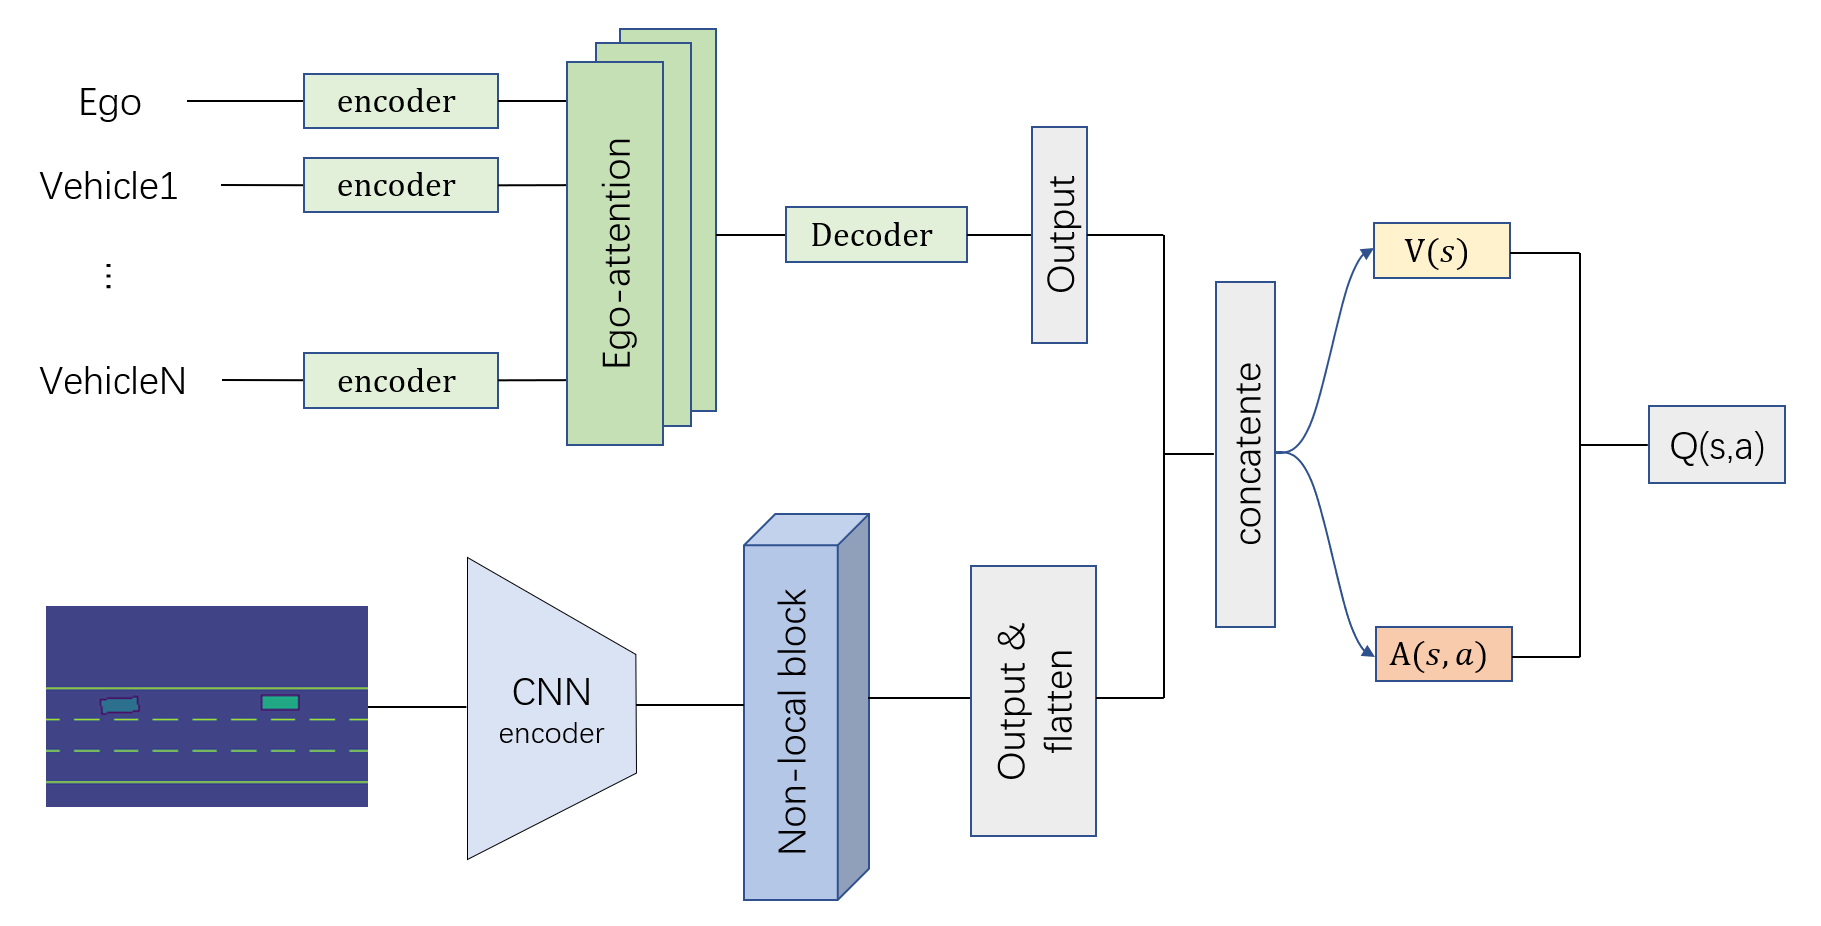
\includegraphics[width=\linewidth]{fig/总体架构.png}
    \caption{基于注意力机制的Dueling DDQN网络框架\cite{wang2021highway}}
    \label{fig:总体架构}
  \end{figure}

\subsection{Ego-attention}
对于基于向量的状态输入,这里采用的注意力模型是ego-attention\cite{leurent2019social}。这种注意力模型是社会注意力机制的一种变形,可以使得智能体更加关注距离其较近或者容易发生碰撞的车辆。

基于ego-attention注意力机制的模型如图\ref{fig:ego-attention}所示,其可以用来表示DQN算法或者Dueling DDQN算法中的Q函数。
\begin{figure}[htbp]
    \centering
    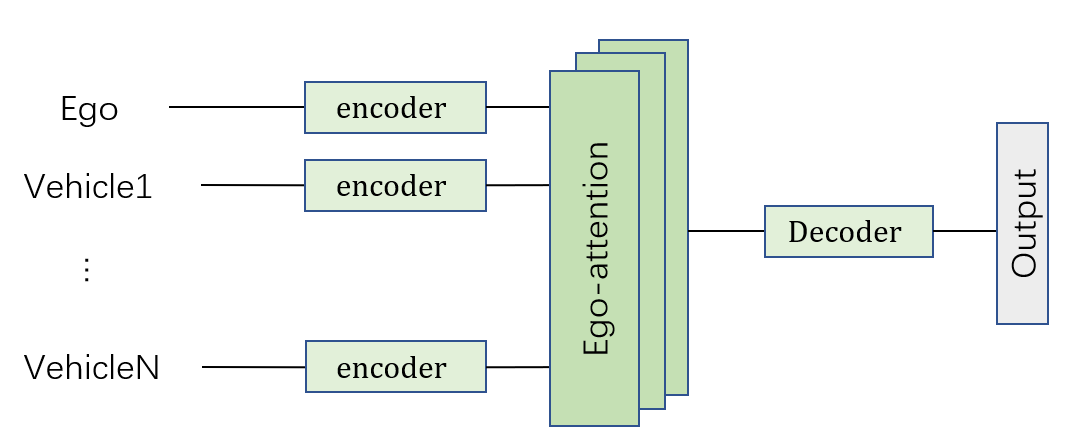
\includegraphics[width=\linewidth]{fig/ego-attention网络结构}
    \caption{基于ego-attention的网络结构}
    \label{fig:ego-attention}
  \end{figure}
网络首先由线性编码层组成,所有编码层的权重相同。经过线性编码层后每个实体
的特征维度为$d_x$,编码后的特征送入由多头堆叠而成的ego-attention层。该层类似于多头自注意力层\cite{vaswani2017attention}但是仅有关于当前车辆的单个输出,也即仅有当前车辆的询问编码。
Ego-attention头的结构如图\ref{fig:ego-head}所示,
\begin{figure}[htbp]
    \centering
    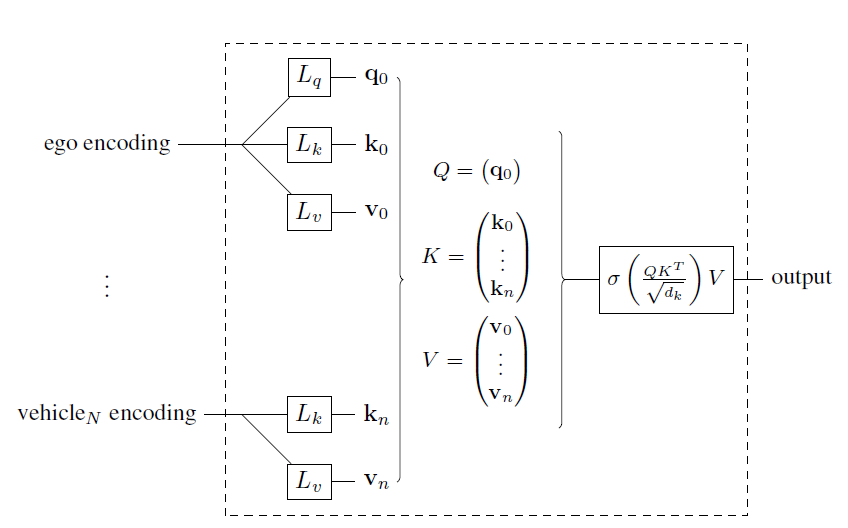
\includegraphics[width=\linewidth]{fig/ego-attention结构.png}
    \caption{ego-attention头的结构}
    \label{fig:ego-head}
  \end{figure}
  为了选择基于环境车辆的子集,当前实体首先发出单个询问$Q=[q_0]\in \mathbb{R} ^{1\times d_k}$,由当前实体编码特征经过线性投影
$L_q\in\mathbb{R} ^{d_x\times d_k}$。这个询问之后与键的集合$K=[k_0,\ldots,k_N]\in\mathbb{R} ^{N\times d_k}$进行比较,其中包含每个实体的描述性特征$k_i$,同样是由
共享权重的线性映射$L_k\in\mathbb{R} ^{d_x\times d_k}$计算得到。询问$q_0$与任意键$k_i$间的相似性由它们之间的点积$q_0k_i^T$衡量,并由$1/\sqrt{d_k}$进行放缩,最后由softmax算子$\sigma $进行归一化。
得到的注意力矩阵用来对输出值的集合$V=[v_0,\ldots,v_N]$进行加权融合,其中每个值$v_i$是经过共享权重的线性映射$L_v\in\mathbb{R} ^{d_x\times d_v }$得到的特征。
综上,每头的注意力计算可以写作:
\begin{equation}
    output=\sigma\left(\frac{QK^T}{\sqrt{d_k}}\right)V
    \label{con:output}
\end{equation}

最后所有头的输出经过一个线性层进行结合,整个过程具有置换不变性:一个置换$\tau$会改变公式中键$K$与值$V$行的顺序,但是两者的对应关系仍然得以保持。它也可以很自然地解释当前车辆与环境车辆的交互关系。

\subsection{Non-local block}
对于基于图像的状态输入,这里使用的注意力机制为non-loacl block\cite{wang2018non}。传统的卷积网络是处理局部区域的操作,为了从图像中获得较大范围的信息,需要通过叠加多层卷积来不断扩大感受野,这样的操作是复杂的,而且需要考验网络设计能力,最终得到的效果也不尽如人意,很难获得较大距离像素间的相对关系。受计算机视觉中非局部均值(non-local means)的启发,non-local block被提出用于捕捉长距离依赖,与传统的卷积神经网络相比,它可以计算两个任意位置之间的交互,进而直接捕获长距离的依赖关系。另外,这一操作是非保持了输入输出的大小,可以很容易地作为一个模块与其他操作结合。

\begin{figure}[htbp]
    \centering
    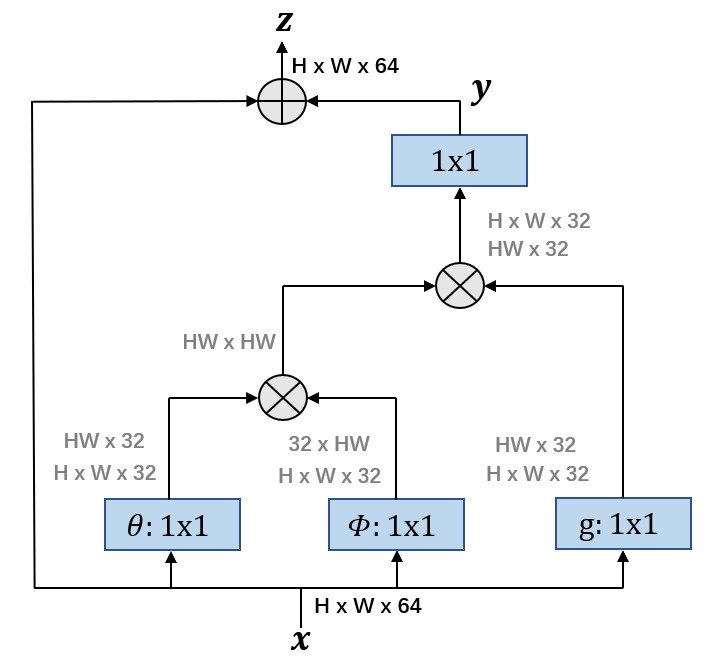
\includegraphics[width=\linewidth]{fig/non-local细节.png}
    \caption{non-local block网络结构}
    \label{fig:nonlocal block}
  \end{figure}
在本文中使用的non-local block如图\ref{fig:nonlocal block}所示,$x$是输入,$z$是non-local block的输出,$y$是non-local操作的结果,其关系式为:
\begin{equation}
    z_i=W_z*y_i + x_i
\end{equation}
$W$是对$y_i$的加权,与输入$x$相加形成残差连接。
\begin{equation}
    y_i = \frac{1}{C(x)}\sum_{\forall j}f(x_i,x_j)g(x_j)
\end{equation}
$f(x_i,x_j)$用来计算$i$和所有可能关联的位置$j$之间的关系,其计算方式可以有多种,在本文中我们使用简单的点乘,如式\ref{f函数};$g(x_j)$用于计算输入信号在$j$位置的特征值;$C(x)$是归一化参数。
\begin{equation}\label{f函数}
    f(x_i,x_j)=\theta(x_i)^{T}\phi(x_j)
\end{equation}
$\theta(x_i)$、$phi(x_j)$、$g(x_j)$均为线性变换,通过空间$1*1$的卷积实现。


基于non-loacl block机制,图片作为状态输入的网络模型如图\ref{fig:基于non-local block的网络结构}所示,与上文的ego-attention模型相似,基于non-local block的网络可以用来拟合DQN算法或者Dueling DDQN算法中的Q函数。网络输入包括当前车辆和环境车辆的为图像信息,通过一个浅层的CNN网络初步提取图像特征,然后使用non-local block提取任意两个像素之间的依赖关系,从而获得当前车辆与环境车辆之间的关系。
\begin{figure}[htbp]
    \centering
    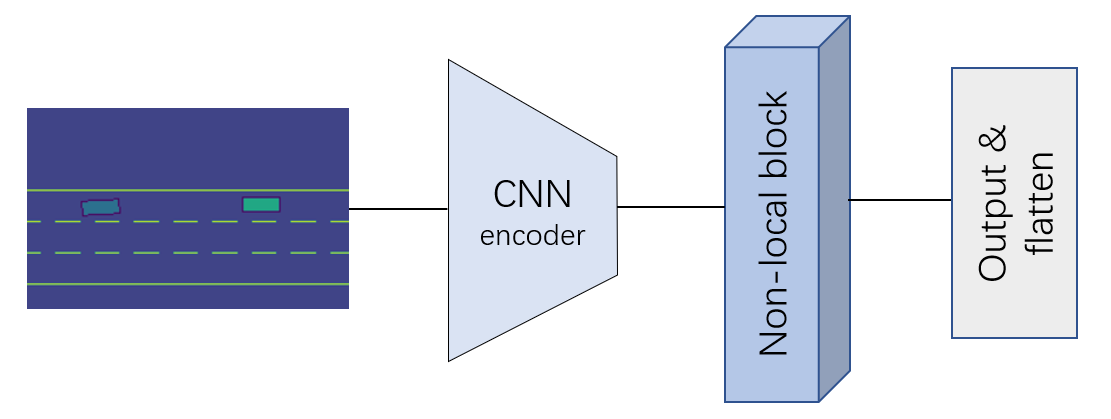
\includegraphics[width=\linewidth]{fig/non-local网络.png}
    \caption{引入non-local block的网络结构}
    \label{fig:基于non-local block的网络结构}
  \end{figure}


\section{实验分析}
在实验部分,我们将奖励函数分为三个部分
\begin{enumerate}
    \item 安全项:碰撞惩罚-1,无碰撞为0
    \item 效率项:令$r_v = 0.4\frac{(v_t-v_{min})}{(v_{max}-v_{min})}$其中,$v_{max} = 30m/s,v_{min}=20m/s$
    \item 靠右项:如果靠右行驶,则奖励为0.1,否则为0
\end{enumerate}

最终的奖励函数为三者的叠加。下面我们将针对不同输入,不同奖励函数设置,不同算法进行一系列的对比试验。同时将我们的带有死亡判断的D3QN进行消融实验,以验证我们算法的有效性。
\subsection[]{不同输入}
我们分别尝试了向量输入、图像输入、和混合输入三种形式。并且针对他们是否加上注意力机制方法进行了广泛地比较。训练1000轮之后进行测试,测试结果取十次测试的平均成绩。最终结果如表\ref{inputtable}所示:
\begin{table}[!htbp] 
    \centering
    \caption{不同输入结果比较}
    \begin{tabular}{ccccccccccc} %需要10列
    \toprule %添加表格头部粗线
    \multicolumn{3}{c}{输入类型}& 步长& 奖励&换道次数&安全率\\
    \hline %绘制一条水平横线
    \multicolumn{3}{c}{向量}& 49.1& 38.19& 16.4 &0.9& \\   % 占两列,列名为A;后面陆续跟着数字
    \multicolumn{3}{c}{图像}& 49.5& 44.4& 23.5 &0.9& \\
    \multicolumn{3}{c}{向量+注意力}& 50.0& 36.5& 46.1 &1.0& \\
    
    \multicolumn{3}{c}{图像+注意力}& 43.4& 39.3& 7.7 & 0.7& \\
    \multicolumn{3}{c}{混合+注意力}& 50.0& 43.1& 9.5 &1.0& \\
    \bottomrule %添加表格底部粗线
    \end{tabular}   
    \label{inputtable} 
\end{table}

经过对比我们可以发现在加入注意力机制之后,可能会导致某些指标改善(如安全率,换道次数),但是也同时会导致一些指标的下降。而且在单一输入情况下,控制效果不稳定,可能导致结果方差较大。比如纯图像输入虽然在此轮测试中奖励最高,但是不稳定,有时平均奖励会到35左右。

这也许是因为注意力机制本身会导致网络收敛震荡,而且单一输入情况下,信息不完全,导致这种震荡更加明显。混合输入的注意力机制方法具有较强的稳定性,同时能够显著提升回报成绩。

\subsection[]{更改奖励系数}
我们针对奖励系数,分别将效率项奖励系数变化为0.2,0.6。将靠右行驶奖励分别变为0和0.2.来验证奖励系数对于车辆控制效果的影响。训练方法采用我们上个实验表现最好的混合输入+注意力机制方法。同样我们训练1000轮之后测试10轮取平均成绩,值得提出的是,在测试过程中我们采用的是同一奖励函数,即最原始的奖励函数来保证我们的实验结果有可对照性。最终结果如表\ref{reward}。

\begin{table}[!htbp] 
    \centering
    \caption{不同奖励函数结果比较(测试时奖励函数相同)}
    \begin{tabular}{ccccccccccc} %需要10列
    \toprule %添加表格头部粗线
    \multicolumn{3}{c}{奖励函数设置}& 步长& 奖励&换道次数&安全率\\
    \hline %绘制一条水平横线
    \multicolumn{3}{c}{增大效率奖励}& 48.6& 44.7& 5.6 &0.8& \\   % 占两列,列名为A;后面陆续跟着数字
    \multicolumn{3}{c}{减小效率奖励}& 50.0& 40.53& 42.6&1.0& \\
    \multicolumn{3}{c}{增大靠右奖励}& 42.0& 38.92& 16.4 & 0.5& \\
    \multicolumn{3}{c}{移去靠右奖励}& 49.4& 41.06& 18.6 &0.9& \\
    \multicolumn{3}{c}{原方案对照}& 50.0& 43.1& 9.5 &1.0& \\
    \bottomrule %添加表格底部粗线
    \end{tabular}   
    \label{reward} 
\end{table}

根据结果可以得到,单纯增大效率奖励系数会使整个车辆控制更加激进,显著减小换道次数,增大速度。但是与此同时,车辆的安全性也会降低。反之减小效率奖励会使整个控制的安全性增大,但是车辆控制会趋于保守,换道次数明显增加、速度也会变慢。

针对靠右奖励而言,移去靠右奖励之后,换道次数有小幅上升,但是由于靠右奖励本身系数较小,因此对于整体效果影响没有增大效率项这么明显。而如果过于增大靠右奖励,将导致网络在靠右和躲避车辆之间权衡被打破,反而会降低效果。

\subsection[]{更改训练算法}
同时我们还验证了不同算法对于结果的影响,分别采用了DQN,DDQN,Dueling DQN与我们的算法进行比较,同样也是训练1000轮之后测试10轮取平均值,最终结果如表\ref{aldif}。

\begin{table}[!htbp] 
    \centering
    \caption{不同训练算法结果比较}
    \begin{tabular}{ccccccccccc} %需要10列
    \toprule %添加表格头部粗线
    \multicolumn{3}{c}{训练算法}& 步长& 奖励&换道次数&安全率\\
    \hline %绘制一条水平横线
    \multicolumn{3}{c}{DQN}& 49.5& 46.44& 23.7 &0.9& \\   % 占两列,列名为A;后面陆续跟着数字
    \multicolumn{3}{c}{DDQN}&48.8& 36.83& 45.1&0.9& \\
    \multicolumn{3}{c}{Dueling DQN}& 46.5& 41.09& 9.3 & 0.9& \\
    \multicolumn{3}{c}{原方案对照}& 50.0& 43.1& 9.5 &1.0& \\
    \bottomrule %添加表格底部粗线
    \end{tabular}   
    \label{aldif} 
\end{table}

经过对比发现,D3QN算法在稳定性和训练效果方面都是目前而言最佳的。其余方法可能导致换道次数显著上升。

\subsection[]{死亡判断对结果影响}
为了验证死亡判断对于网络的影响,我们对比了是否加入死亡判断对于最终训练结果的影响。其余设置条件均相同,最终结果如表\ref{deadnot}所示。
\begin{table}[!htbp] 
    \centering
    \caption{是否加入死亡判断结果比较}
    \begin{tabular}{ccccccccccc} %需要10列
    \toprule %添加表格头部粗线
    \multicolumn{3}{c}{是否加入死亡判断}& 步长& 奖励&换道次数&安全率\\
    \hline %绘制一条水平横线
    \multicolumn{3}{c}{否}& 42.7& 35.91& 20.9 &0.8& \\   % 占两列,列名为A;后面陆续跟着数字
    \multicolumn{3}{c}{原方案对照}& 50.0& 43.1& 9.5 &1.0& \\
    \bottomrule %添加表格底部粗线
    \end{tabular}   
    \label{deadnot} 
\end{table}

根据实验结果可以很明显看到,加入死亡判断对于最终结果有一个很明显的提升

\section{结论}
在本次工作中,我们提出基于注意力机制的加入死亡判断的Dueling DDQN强化学习算法,为自动驾驶车辆超车换道提供最优的行动决策。采用向量和图像作为混合输入,针对向量形式的状态输入,构建了基于ego-attention的子网络,有效提取当前车辆和环境车辆的交互关系;针对图像形式的状态输入,构建了基于non-local block的子网络,通过non-local操作,直接捕获图像中不同车辆之间的依赖关系。为验证所提方法的优越性,我们对不同输入、不同奖励函数设置、不同算法进行了一系列对比实验。实验结果表明,加入注意力机制后,车辆换道的总体控制效果得到提高;相比于单输入的情况,混合输入能够引入更全面的信息,使得训练结果更加稳定。增大效率奖励系数可以获得更大的奖励,但安全性会稍有下降;减小效率奖励系数后,车辆的控制趋于保守,换道次数明显增加,速度也会变慢,这和我们的经验也是相符的。适当的靠右奖励可以减少车辆换道次数,过大或移去靠右奖励都会降低控制效果。与DQN、DDQN、Dueling DQN相比,所提出的方法在步长、奖励、换道次数、安全率等方面均获得了最优的效果。与不具备死亡判断的方法相比,所提方法在各指标中均有显著提升,体现了死亡判断对训练效果提升的重要作用。总之,所提出的基于注意力机制的加入死亡判断的Dueling DDQN强化学习算法在各方面表现最优,能够有效控制自动驾驶车辆安全换道。

需要说明的是,我们发现多次训练后的模型获得的测试结果并不稳定,所以在本文中报告的实验数据均为相对平均或者低于平均的保守结果,更加鲁棒的控制算法可能是我们今后需要继续深入研究的一个方向。

\addtolength{\textheight}{-1cm}   % This command serves to balance the column lengths
                                  % on the last page of the document manually. It shortens
                                  % the textheight of the last page by a suitable amount.
                                  % This command does not take effect until the next page
                                  % so it should come on the page before the last. Make
                                  % sure that you do not shorten the textheight too much.

%%%%%%%%%%%%%%%%%%%%%%%%%%%%%%%%%%%%%%%%%%%%%%%%%%%%%%%%%%%%%%%%%%%%%%%%%%%%%%%%



%%%%%%%%%%%%%%%%%%%%%%%%%%%%%%%%%%%%%%%%%%%%%%%%%%%%%%%%%%%%%%%%%%%%%%%%%%%%%%%%



%%%%%%%%%%%%%%%%%%%%%%%%%%%%%%%%%%%%%%%%%%%%%%%%%%%%%%%%%%%%%%%%%%%%%%%%%%%%%%%%
%\section*{APPENDIX}

%Appendixes should appear before the acknowledgment.

\section*{小组分工}
沈炼成主要负责了仿真环境和基础训练算法搭建,林镇阳负责了ego-attention的模块,韩立君负责了non-local block的模块。最后报告由三人合写并修改。




%%%%%%%%%%%%%%%%%%%%%%%%%%%%%%%%%%%%%%%%%%%%%%%%%%%%%%%%%%%%%%%%%%%%%%%%%%%%%%%%

%References are important to the reader; therefore, each citation must be complete and correct. If at all possible, references should be commonly available publications.

\bibliographystyle{unsrt}
\bibliography{ref}%%我们的例子应该是\bibliography{cited}




\end{document}
